\chapter{Material}
\label{ch:Material}
\enlargethispage{120cm}
\section{PMOD-Pinbelegung des IceZero-Boards}

Bei der Pin-Belegung wurde das selbe Schema wie beim GPIO-Modul des IcoSoc verwendet. Die Numerierung läuft dementsprechend von rechts nach links und für die einzelnen PMOD-Header ``zeilenweise'' von oben nach unten.

\begin{figure}[h]
	\centering
	\captionsetup{justification=centering,margin=2cm}
		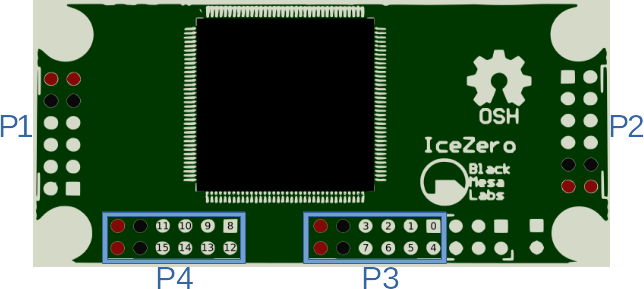
\includegraphics[width=0.80\textwidth]{../figures/ice40_pmod_pins_01.png}
		\caption[Pinbelegung der PMOD-Header des IceZero-Boards]{Pinbelegung der PMOD-Header des IceZero-Boards (Quelle: Eigene Abbildung)}
	\label{fig:ice40_pmod_pins}
\end{figure}

\begin{table}[h]
\centering
\resizebox{\columnwidth}{!}{%
\begin{tabular}{lllllllllllll}
\cline{1-6} \cline{8-13}
\multicolumn{1}{|l|}{\cellcolor[HTML]{DF2727}3.3V} & \multicolumn{1}{l|}{\cellcolor[HTML]{343434}{\color[HTML]{FFFFFF} GND}} & \multicolumn{1}{l|}{pin\_11} & \multicolumn{1}{l|}{pin\_10} & \multicolumn{1}{l|}{pin\_9}  & \multicolumn{1}{l|}{pin\_8}  & \multicolumn{1}{l|}{} & \multicolumn{1}{l|}{\cellcolor[HTML]{DF2727}3.3V} & \multicolumn{1}{l|}{\cellcolor[HTML]{343434}{\color[HTML]{FFFFFF} GND}} & \multicolumn{1}{l|}{pin\_3} & \multicolumn{1}{l|}{pin\_2} & \multicolumn{1}{l|}{pin\_1} & \multicolumn{1}{l|}{pin\_0} \\ \cline{1-6} \cline{8-13} 
\multicolumn{1}{|l|}{\cellcolor[HTML]{DF2727}3.3V} & \multicolumn{1}{l|}{\cellcolor[HTML]{343434}{\color[HTML]{FFFFFF} GND}} & \multicolumn{1}{l|}{pin\_15} & \multicolumn{1}{l|}{pin\_14} & \multicolumn{1}{l|}{pin\_13} & \multicolumn{1}{l|}{pin\_12} & \multicolumn{1}{l|}{} & \multicolumn{1}{l|}{\cellcolor[HTML]{DF2727}3.3V} & \multicolumn{1}{l|}{\cellcolor[HTML]{343434}{\color[HTML]{FFFFFF} GND}} & \multicolumn{1}{l|}{pin\_7} & \multicolumn{1}{l|}{pin\_6} & \multicolumn{1}{l|}{pin\_5} & \multicolumn{1}{l|}{pin\_4} \\ \cline{1-6} \cline{8-13} 
\multicolumn{6}{c}{PMOD - P4}                                                                                                                                                                                                                            &                       & \multicolumn{6}{c}{PMOD - P3}                                                                                                                                                                                                                      
\end{tabular}
}
\caption{Pinbelegung der PMOD-Header des Icezero-Boards}
\label{tbl:PMOD-Pins}
\end{table}


\clearpage
\begin{landscape}

\section{Pinverbindungen Raspberry Pi und FPGA-Shield}

\begin{table}[h]
\centering
\caption{Pinbelegung}
\label{tbl:Pinbelegung}
\begin{tabular}{|l|l|l|
>{\columncolor[HTML]{EFEFEF}}l |
>{\columncolor[HTML]{EFEFEF}}l |l|l|l|}
\hline
\cellcolor[HTML]{C0C0C0}ice40 & \cellcolor[HTML]{C0C0C0}WiringP & \cellcolor[HTML]{C0C0C0}Name                       & \multicolumn{2}{l|}{\cellcolor[HTML]{C0C0C0}Physical} & \cellcolor[HTML]{C0C0C0}Name                       & \cellcolor[HTML]{C0C0C0}WiringPi & \cellcolor[HTML]{C0C0C0}ice40 \\ \hline
                              &                                 & \cellcolor[HTML]{DF2727}3.3V                       & 1                         & 2                         & \cellcolor[HTML]{DF2727}5V                         &                                  &                               \\ \hline
                              & 8                               & SDA.1                                              & 3                         & 4                         & \cellcolor[HTML]{DF2727}5V                         &                                  &                               \\ \hline
                              & 9                               & SCL.1                                              & 5                         & 6                         & \cellcolor[HTML]{000000}{\color[HTML]{FFFFFF} GND} &                                  &                               \\ \hline
                              & 7                               & 1-Wire                                             & 7                         & 8                         & TxD                                                & 15                               &                               \\ \hline
                              &                                 & \cellcolor[HTML]{000000}{\color[HTML]{FFFFFF} GND} & 9                         & 10                        & RxD                                                & 16                               &                               \\ \hline
                              & 0                               & GPIO. 0                                            & 11                        & 12                        & GPIO.1                                             & 1                                &                               \\ \hline
                              & 2                               & GPIO. 2                                            & 13                        & 14                        & \cellcolor[HTML]{000000}{\color[HTML]{FFFFFF} GND} &                                  &                               \\ \hline
                              & 3                               & GPIO. 3                                            & 15                        & 16                        & GPIO. 4                                            & 4                                &                               \\ \hline
                              &                                 & \cellcolor[HTML]{DF2727}3.3V                       & 17                        & 18                        & GPIO. 5                                            & 5                                &                               \\ \hline
                              & 12                              & MOSI                                               & 19                        & 20                        & \cellcolor[HTML]{000000}{\color[HTML]{FFFFFF} GND} &                                  &                               \\ \hline
                              & 13                              & MISO                                               & 21                        & 22                        & GPIO. 6                                            & 6                                &                               \\ \hline
                              & 14                              & SCLK                                               & 23                        & 24                        & CE0                                                & 10                               &                               \\ \hline
                              &                                 & \cellcolor[HTML]{000000}{\color[HTML]{FFFFFF} GND} & 25                        & 26                        & CE1                                                & 11                               &                               \\ \hline
                              & 30                              & SDA.0                                              & 27                        & 28                        & SCL.0                                              & 31                               &                               \\ \hline
			      & 21                              & GPIO.21                                            & 29                        & 30                        & \cellcolor[HTML]{000000}{\color[HTML]{FFFFFF} GND} &                                &                               \\ \hline
                              & 22                              & GPIO.22                                            & 31                        & 32                        & GPIO.26                                            & 26                               &                               \\ \hline
                              & 23                              & GPIO.23                                            & 33                        & 34                        & \cellcolor[HTML]{000000}{\color[HTML]{FFFFFF} GND} &                                &                               \\ \hline
                              & 24                              & GPIO.24                                            & 35                        & 36                        & GPIO.27                                            & 27                               &                               \\ \hline
                              & 25                              & GPIO.25                                            & 37                        & 38                        & GPIO.28                                            & 28                               &                               \\ \hline
                              &                                 & \cellcolor[HTML]{000000}{\color[HTML]{FFFFFF} GND} & 39                        & 40                        & GPIO.29                                            & 29                               &                               \\ \hline
\end{tabular}
\end{table}
\end{landscape}

\clearpage

\section{CD}
Die beiliegende CD enthält den Inhalt des Github-Repositories 
\begin{lstlisting}[language=bash]
https://github.com/dm7h/fpga-event-recorder
\end{lstlisting}
zum Zeitpunkt der Abgabe.

Folgende Tabelle entält einen Überblick über die Inhalte des Repositories:
\begin{table}[h]
\centering

\begin{tabular}{|p{1cm}|p{3cm}|p{10cm}|}
\hline
\rowcolor[HTML]{C0C0C0} 
Verz. & Unterverzeichnis                & Inhaltsbeschreibung                                                                                                                                                                                                                                                                                                      \\ \hline
doc/        & ref/                            & iCE40 Manuals und relevante Hardwaredokumentation                                                                                                                                                                                                                                                                        \\ \hline
thesis/     &                                 & Finale Version der Bachelorarbeit als PDF                                                                                                                                                                                                                                                             \\ \hline
thesis/     & src/                            & Latex-Sourcen der Bachelorarbeit                                                                                                                                                                                                                                                              \\ \hline
src/        &                                 &                                                                                                                                                                                                                                                                                                                          \\ \hline
            & Logikanalysator/                & Dateien des Semesterprojekts ``Logikanalysator mit AVR Mega32U4 und Altera MAX CPLD''  inkl. Dateien der Bachelorarbeit von Andreas Müller (USB-TPLE)  
															     \\ \hline
            & icotools/                       & Portierung des icotools Projekts für das IceZero-Board. Original-Repository: https://github.com/cliffordwolf/icotools. Relevant sind hier vor allem die Unterverzeichnisse ``icosoc'' und ``icoprog'' 
\\ \hline
            & icozctl/                        & Fork des icoprog-Tools (icotools/icoporg) mit zusätzlichen Funktionen zur Steuerung des Event-Recorders                                                                                                                                                                                                                  \\ \hline
            & icozero/                        & Vom IcoSoc unabhängiges Beispiel-Projekt für das IceZero-Board mit leichten Modifikationen (nicht projekt-relevant)                                                                                                                                                                                                      \\ \hline
            & picosoc/                        & Portierung des PicoSoc-Projekts auf das IceZero-Board (nicht direkt projekt-relevant). PicoSoc ist eine minimale Variante des IcoSocs. Original-Repository: https://github.com/cliffordwolf/picorv32/tree/master/picosoc                                                    \\ \hline
            & sump2/                          & SUMP2 Variante für das IceZero-Board (nicht für die Icestorm-Toolchain)                                                                                                                                                                                                                                                  \\ \hline
            & sump2\_pipistrello\_ ftdi\_fifo/ & SUMP2 Vairante für das Pipistrello-Board bei dem der Versuch unternommen wurde den UART durch einen FTDI-Fifo zu ersetzen, um einen Höheren Datenduchsatz zu ermöglichen. Quelle: http://forum.gadgetfactory.net/topic/1748-open-bench-logic-sniffer-with-64mb-capture-buffer/ \\ \hline
            & demon-core-import/              & SUMP2 Weiterenwicklung für den Open Bench Logic Sniffer. Quelle: https://github.com/jhol/demon-core-import                                                                                                                                                                     \\ \hline
\end{tabular}
\caption{Überblick über den Inhalt des Git-Repositories}
\label{tbl:git_repo}
\end{table}
